\documentclass{siproblemset}

\usepackage{multicol}
\usepackage{xcolor}

% SI Session Information
\course{MTH 1321}
\sessionnum{3}
\sessiondate{1/23/20}

\warmup{Concept Review}
\topic{What is a limit?}
\topic{Recognizing Continuity}
\topic{Determining Continuity}
\cooldown{Challenge Problems}

% Worksheet Information
\title{Continuity, Limits of \linebreak Continuous Functions}
\sections{Sections 2.4a}
\withnamespace

\begin{document}
    \maketitle
    
    \activity{Warmup}{Concept Overview}{Work \textbf{alone} then share your answers with a \textbf{partner}. Try not to use your notes.}{15 minutes}
    
    \frq{Define continuity in your own words and give the formal definition.}
    \Tinysp
    
    \frq{Give the formal definition of left- and right-continuity.}
    \Tinysp
    
    \frq{Name the three common types of discontinuities and sketch an example (graph) of each.}
    \Smallsp
    
    \frq{Name some of the basic functions which are continuous on their domains.}
    \Smallsp
    
    \pagebreak
    \activity{Activity 1}{Determining Continuity}{Work in a \textbf{group of 2 or 3 people sitting near you} to answer these questions. Try not to use your notes.}{30 minutes}
    
    \begin{multipartquestion}
        Determine the intervals of continuity on the following graphs. At points of discontinuity, state if the function is left- or right-continuous at that point and the type of discontinuity.
        \frq{}
        \mbox{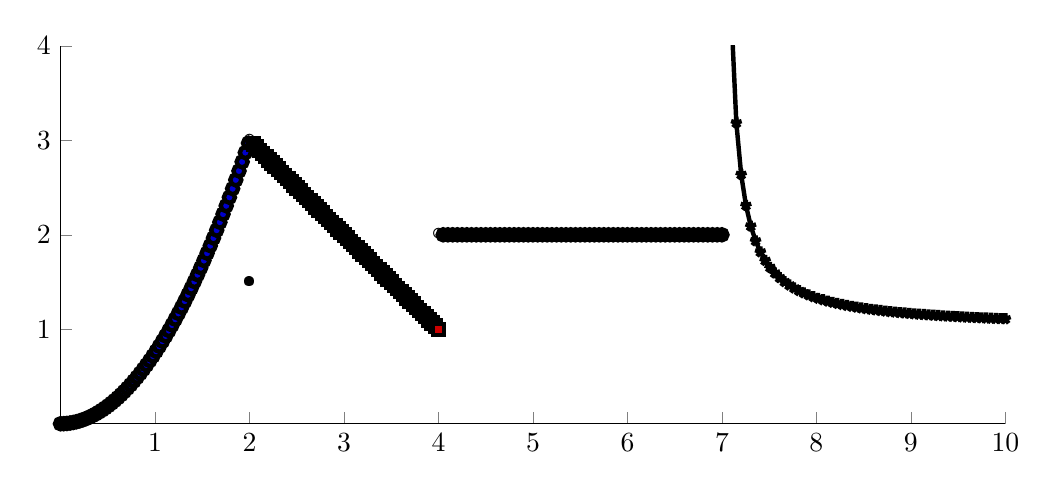
\begin{tikzpicture}[baseline=(current bounding box.north)]
            \begin{axis}[
                x=1.2cm,
                y=1.2cm,
                xmin=0,
                xmax=10,
                ymin=0,
                ymax=4,
                axis x line*=middle,
                axis y line*=middle,
                every axis plot/.append style={ultra thick},
                samples=60
                ]
                \addplot+[black, domain=0:1.99] {3/4*x^2};
                \node at (2,3) {$\circ$};
                \node at (2,1.5) {\textbullet};
                \addplot+[black, domain=2.04:4] {-x+5};
                \node at (4,1) {\textbullet};
                \node at (4,2) {$\circ$};
                \addplot+[black, domain=4.05:7] {2};
                \node at (7,2) {\textbullet};
                \addplot+[black, domain=7:10] {1/(3*(x-7))+1};
            \end{axis}
        \end{tikzpicture}}
        \tinyspace
        \frq{}
        \mbox{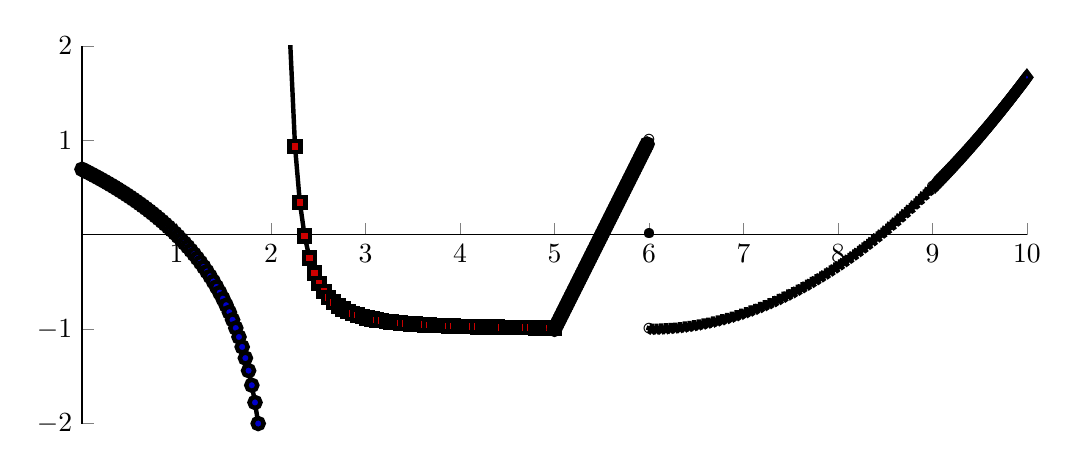
\begin{tikzpicture}[baseline=(current bounding box.north)]
            \begin{axis}[
            x=1.2cm,
            y=1.2cm,
            xmin=0,
            xmax=10,
            ymin=-2,
            ymax=2,
            axis x line*=middle,
            axis y line*=middle,
            every axis plot/.append style={ultra thick},
            samples=60
            ]
            \addplot+[black, domain=0:2] {ln(-(x-2))};
            \addplot+[black, domain=2:5,restrict y to domain =-5:5] {1/(8*(x-2)^2)-1};
            \node at (5,-1) {\textbullet};
            \addplot+[black, domain=5:5.98] {2*x-11};
            \node at (6,1) {$\circ$};
            \node at (6,0) {\textbullet};
            \node at (6,-1) {$\circ$};
            \addplot+[black, domain=6.03:8.97] {1/6*(x-6)^2-1};
            \node at (9,0.5) {$\circ$};
            \addplot+[black, domain=9.03:10] {1/6*(x-6)^2-1};
            \end{axis}
            \end{tikzpicture}}
        \tinyspace
    \end{multipartquestion}
    \pagebreak
    
    \mcq{Use the limit properties and definition of continuity to determine if the following functions are continuous at the specified points. If they are not, determine if they are left or right continuous at those points. Justify your answers.}{
        \task $f(x)=\dfrac{4x+5}{9-3x} ~;~ x=-1$
        \Smallsp
        \task $g(x)=\begin{cases}
        2x & x < 6 \\
        x-1 & x\geq 6
        \end{cases} ~;~ x=6$
        \Smallsp
        \task $h(z)=\dfrac{5z-20}{z^2-12z} ~;~ z=0$
        \Smallsp
        \task $l(x)=\begin{cases}
        e^x+\sin(x)-2 & x \leq 2\\
        x^2 &x > 2
        \end{cases} ~;~ x=4$ 
    }

    \pagebreak
    \activity{Activity 2}{Limits of Continuous Functions and Indeterminate Forms}{Work in a \textbf{group of 2 or 3 people with the same color worksheet as you} to answer these questions. Try not to use your notes.}{30 minutes}
    
    \mcq[2]{Find the points of discontinuity of the given function. State the type of discontinuity and if the function is left- or right-continuous at those point(s). If there are no points of discontinuity, state so explicitly. Justify your answers.}{
%        \task $h(x)=\dfrac{1}{x+5}$
%        \normalsp
        \task $g(x)=\dfrac{x+2}{3-x}$
        \hugesp
%        \task $s(t)=\tan(t) ~;~ -\pi< t<\pi$
%        \normalsp
        \task $a(b)=\dfrac{1}{b^2-9}$
        \hugesp
        \task $f(x)=\cos(\sin x)$
        \hugesp
        \task $b(z)=\ln|z+2|$
        \hugesp
%        \pagebreak
        \task $f(x)=\sqrt{x^2-2}$
        \hugesp
        \task $h(x)=\begin{cases}
        x^2 & x < 1\\
        4-3x &1 \leq x \leq 2\\
        \sqrt{x-2} & x < 2
        \end{cases}$ 
        \hugesp
    }
    
    \activity{Cooldown}{Challenge Problems}{Test your knowledge of recent topics by attempting these challenge problems \textbf{alone} then sharing your answers with the people around you.}{15 minutes}
    
    \frq{What are $\lim\limits_{x\to c^\pm}f(x)$ and $f(c)$ for each type of discontinuity?}
    \pagebreak
    
    \begin{multipartquestion}
        Are the following functions continuous at $x=k$? If they are not, state the type of discontinuity and whether the function is left- or right-continuous (or neither) at $x=k$.
        \frq{$h(k)=5~;~\lim\limits_{x\rightarrow k^+}h(x)=5~;~\lim\limits_{x\rightarrow k^-}h(x)=2$}
        \Smallsp
        \frq{$f(k)=4~;~\lim\limits_{x\rightarrow k}f(x)=4$}
        \Smallsp
        \frq{$g(k)=6~;~\lim\limits_{x\rightarrow k}g(x)=-2$}
        \Smallsp
        \frq{$q(k)=3~;~\lim\limits_{x\rightarrow k^+}q(x)=-6~;~\lim\limits_{x\rightarrow k^-}q(x)=-\infty$}
        \Smallsp
    \end{multipartquestion}
\end{document}